%************************************************
\chapter[Behaviour and life history in novel environments]{Behaviour, life
history and persistence in novel environments
  \footnote{Published in: Maspons, J., R. Molowny‐Horas, \& D. Sol. 2019. Behaviour, life
  history and persistence in novel environments. \textit{Phyl. Trans. R. Soc. B}
  374:20180056.
  \href{http://dx.doi.org/10.1098/rstb.2018.0056}{doi:10.1098/rstb.2018.0056}
  }
}\label{ch:LH-Behaviour model}
%************************************************


\section*{Abstract}

Understanding what affects population growth in novel environments is
fundamental to forecast organisms’ responses to global change, including
biological invasions and land use intensification. Novel environments are
challenging because they can cause maladaptation, increasing the risk of
extinction by negative population growth. Animals can avoid extinction by
improving the phenotype–environment match through behavioural
responses, notably matching habitat choice and learning. However, the 
demographic consequences of these responses remain insufficiently understood in
part because they have not been analysed within a life-history context. By
means of an individual-based model, we show here that matching habitat
choice and learning interact with life history to influence persistence in
novel environments. In maladaptive contexts, the likelihood of persisting is
higher for life-history strategies that increase the value of adults over the
value of offspring, even at the cost of decreasing reproduction. Such a strategy
facilitates persistence in novel environments by reducing the costs of a 
reproductive failure while increasing the benefits of behavioural responses. Our
results reinforce the view that a more predictive theory for extinction risk
under rapid environmental changes requires considering behavioural
responses and life history as part of a common adaptive strategy to cope
with environmental changes.
This article is part of the theme issue ``Linking behaviour to dynamics of
populations and communities: application of novel approaches in behavioural
ecology to conservation''.

\bigskip
\textbf{Keywords:} Biological invasions, Extinction risk, Demographic
stochasticity, Cognitive ecology, Habitat selection, Urbanization

\clearpage


\section{Introduction}

Most organisms experience serious difficulties when exposed to novel
environments. Novel contexts often generate mismatches between the phenotype and
the environment, leading to maladaptation and extinction through negative
population growth \citep{Bell2017}. Maladaptation is one of the reasons why translocations
of species from their native ranges to novel environments generally fail to establish
self-sustaining populations \citep{Sol2016, Sakai2001a}, and it is also a primary cause of extinction by
land use intensification \citep{Sih2011}. Given that biotic exchanges and land use
intensification are becoming increasingly frequent as a result of human activities, there is an
urgent need to understand the mechanisms that influence population persistence
in novel environments.

Several processes can allow organisms to improve the matching of their
phenotypes to new contexts and hence facilitate persistence in novel environments.
Natural selection—the most obvious process—can contribute to
reconstitute the phenotype–environment match through genetic changes, a process
known as evolutionary rescue \citep{Bell2017}. However, an evolutionary rescue is less
effective in animals with long generation time, such as many birds and mammals,
which exhibit slow evolutionary responses to selection. In these animals, behavioural
responses are an alternative to reduce the phenotype–environment
mismatch \citep{Sih2011, Klopfer1981, Sol2003a, Tuomainen2011, Kokko2001}. Individuals may, for instance, improve fitness in novel environments
by choosing the habitats where they live and reproduce that best fit their
phenotype, a process known as matching habitat choice \citep{Nicolaus2018, Stamps2007, Greene2001, Schmidt2010}. Animals can
also decide when is best to reproduce, and skip reproduction
when conditions are unfavourable \citep{williams1966adaptation}.

The choice of where and when to live and reproduce can
express activational plasticity, that is, an innate response to
environmental cues \citep{Snell-Rood2013, Sol2013a}. In a novel environment, however,
individuals must often take decisions with insufficient information
and using cues that may have changed relative to
those from the old environment, which can lead them
to settle in poor-quality habitats (ecological traps) \citep{Kokko2001}. Yet,
animals can improve decision-making, and hence avoid
extinction, through learning \citep{Grieco2002, Kawecki2010}. Learning can modify
decision-making based on previous experiences of the individual \citep{Baudains2007, Eliassen2007}
—for example, changing habitat after a
reproductive failure—or by using public information generated
by more experienced conspecific or heterospecifics
\citep{Doligez2002}. Evidence is accumulating that species which readily
adjust behaviours to novel contexts are better able to survive
and reproduce in a novel environment than species that
persist with the behaviours of their old environments \cite{Kawecki2010, Dukas2008}.

While the importance of behaviour in the response to
environmental changes is widely recognized, we still lack a
general theory regarding how such processes influence
population growth in novel environments \citep{Sol2016}. One important
reason is that behavioural responses have rarely been
investigated within a life-history context \citep{Sol2016, Ricklefs2004}. Life
history—defined as the way organisms distribute their limited
time and energy into growth, reproduction and
survival \cite{stearns1992evolution}—is relevant because it affects how populations
increase and fluctuate over time. The demography of the
organism is particularly influenced by its position in the
fast–slow continuum of life-history variation \cite{Stearns1983a}. Species
at the fast side of the continuum have short life expectancy
but mature early and show high fecundity, which give
them a high potential for rapid population growth under
favourable conditions. Growing fast may confer advantages
during the invasion of novel environments by reducing the
period that the population remains small and hence vulnerable
to extinction by demographic stochasticity. Species at
the slow side of the continuum have delayed maturity and
low fecundity, and hence cannot increase in number so fast
when the population is small. Yet, their long life expectancy
(and long generation time) buffers their populations from
fluctuations driven by demographic and environmental stochasticity
that can lead to extinction \cite{Saether2013, Saether2004}. A slow strategy
also reduces the fitness costs of a reproductive failure, as individuals
have higher chances of breeding again in the future.
This offers advantages in novel environments by spreading
the risk of reproductive failure over several breeding attempts
(a type of bet-hedging) and by allowing individuals to skip a
reproductive event (and hence improve their survival) when
conditions are unfavourable \cite{Sol2012a}.

Thus, when we analyse how behavioural responses affect
the demography of animals in novel, stochastic environments,
we need to be aware that these responses will be affected by the
organism’s life history. This is relevant because the position of
the animal in the fast–slow continuum can alter the benefits
and costs of gathering environmental information and constructing
appropriate behavioural responses \cite{Forcada2008, Saether2000,
Lewontin1969, Saether2005a, Starrfelt2012}. The net
benefit should generally be higher in slow animals, which are
less constrained by time to explore and learn, and can use the
learned behaviours for longer periods. The costs of delaying
reproduction when conditions are unfavourable should also
decrease in slow species, as individuals can reproduce again
in the future, increasing the opportunities for acquiring
environmental information and, through learning, improve
the match of the phenotype to the novel conditions \cite{Sol2012a}.
The demographic consequences of behavioural responses in
novel, stochastic environments are also expected to vary
depending on whether the phenotype–environment mismatch
mainly affects offspring or adult survival. This is because fast
and slow strategies differ in their sensitivity to changes in the
demographic parameters, with fast strategies being highly
sensitive to changes in fecundity and slow strategies to changes
in adult survival \cite{Gaillard2000a}. Thus, understanding how behavioural
responses contribute to population persistence in novel, stochastic
environments requires us to consider the position of
the animal in the fast–slow continuum \citep{Sol2016}.

While the demographic consequences of behaviour have
been previously modelled by several authors \citep{Kokko2001, Cressman2013, Kisdi2002,
kawecki1995demography, Strasser2012}, it
remains to be seen to what extent behavioural responses influence
population growth in novel, stochastic environments as a
function of the position of the animal in the fast–slow continuum.
Here, we use an individual-based simulation model
to address this issue. The behavioural responses that we investigate
include innate preferences for habitats that better
matches the organism’s phenotype, learning rules to reduce
the preference for inadequate habitats and decisions about
skipping a reproductive event when individuals stay in a habitat
that does not match their phenotype. We use the model to
illustrate how considering life-history variation refines predictions
of classic theory regarding the role of behaviour in
facilitating population persistence in novel environments.


\section{Model description}

Building on previous studies \citep{Cressman2013, kawecki1995demography}, we envision a species
that is introduced in a novel region with two habitats.
Individuals are allowed to survive, reproduce and move
between habitats, and the likelihood that the population persists
in the novel region (establishment success) is estimated
through simulations (electronic supplementary material,
figure \ref{fig:figApp3.2.1}). Establishment success is estimated through a
stage-structured population-based model (which allows us
to compare the outcome for species differing in life history),
in scenarios varying in the degree of phenotype–environment
mismatch (causing negative population growth) and
demographic stochasticity (causing extinction by demographic
accidents). The introduced species has a particular
life-history strategy that positions it along the fast–slow continuum,
fixing the values of its onset of first reproduction,
average fecundity and age-specific survival of individuals
(see details below). Behavioural responses are studied by
assessing how modifying the probabilities of changing habitat
and skipping reproduction affects establishment success.
Below, we briefly summarize the main features of the
model. For further details about specific parts of the model
and about its inner workings, we refer the reader to the electronic
supplementary material. The model was built using
the R language \citep{RCoreTeam}, and an accompanying R package implementing
the model, with its corresponding tutorial, is also
offered as the electronic supplementary material at
\url{https://dx.doi.org/10.6084/m9.figshare.c.4546955}.


\subsection*{a) Stage-classified population}

We chose a stage-classification approach to account for the
complex life cycle of our simulated populations. Based on
pre-breeding census, we classify the population into three individual
classes: juveniles, subadults (only for strategies with age
at first reproduction greater than 1 year) and adults. In turn,
adults are divided into non-breeder (i.e. adults that decide
not to breed in a given year) and breeders. Finally, breeding
individuals are split at each brooding step into successful or
failed breeders, distinguishing whether breeding yields viable
juveniles or not, respectively. Only females are considered.


\subsection*{b) Demographic model set-up}

Our population model includes the main processes that must be
considered when evaluating the life cycle of a stage-classified
population, namely survival, growth and reproduction (table \ref{tab:table3.1}):
\begin{description}
  \item[(i) survival:] each stage-class ( juveniles, subadults, non-breeding
    adults and breeding adults) is defined by an annual
    survival rate. In addition, juvenile survival is decomposed
    into individual survival and brood survival, the latter
    affecting all individuals in the same brood (e.g. as a
    result of nest predation). Data about the sources of juvenile
    mortality are scarce, and hence, we fixed the brood level
    mortality to account for 50\% of the juvenile mortality;
  \item[(ii) growth:] individuals can be promoted to the next stage if
    they survive to the next year. Individuals only remain
    1 year in the juvenile class, after which they move up
    to the subadult or adult class. After they reach adulthood,
    they remain in that condition until they die; and
  \item[(iii) reproduction:] each year, the algorithm determines
    which proportion of adults becomes non-breeders or
    breeders, and also which proportion of the latter
    may successfully breed. Only adults that are classified
    at each step as breeders can reproduce during a year.
\end{description}


\begin{table}
\caption[Notation]{Notation followed to describe the stochastic population
model.}\label{tab:table3.1}
\begin{tabular}[b]{@{}p{1.5cm}p{13cm}@{}}
\toprule
\textbf{Symbol} & \textbf{Definition}                                                                                                                                                                                                                                                                                        \\ \midrule
$q$   & Number of offsprings per brood in habitat $h$                                                                                                                                                                                                                                                                        \\
$m$   & Number of broods per year                                                                                                                                                                                                                                                                                            \\
${n}_{Sa}$        & Number of sub-adult stages                                                                                                                                                                                                                                                                               \\
$x$   & Labels for adult breeder type, $x= \{nb, b, b_{s}, b_{f}\}$. Label $nb$ identifies adults that skip breeding and label $b$ indicates adult individuals that try to breed. In turn, the latter can be divided into those which breed successfully (labelled $b_{s}$) or those which fail to do so (labelled $b_{f}$)  \\
$y$   & Labels for survival, $y= \{j, sa, nb, b\}$, where labels refer to juveniles, subadults, non-breeder and breeder adults, respectively                                                                                                                                                                                 \\
$h$   & Index for habitat type, $h= \{1, 2\}$                                                                                                                                                                                                                                                                                \\
$r$   & Label for subadult stage, $r= \{r_{1} \cdots r_{n_{Sa}}\}$                                                                                                                                                                                                                                                           \\
$t$   & Subindex for time steps, measured in years, $t= \{1 \cdots 50\}$                                                                                                                                                                                                                                                     \\
${p}_{h}^{b}$     & Probability for an individual to become a breeder (successful or not) in habitat $h$                                                                                                                                                                                                                     \\
${p}_{h}^{b_{f}}$ & Probability of complete brood failure for a breeder in habitat $h$                                                                                                                                                                                                                                       \\
${p}_{h,S_{x}}$   & Probability of survival in habitat $h$ for individuals $x$                                                                                                                                                                                                                                               \\
$p_{h, s_{y}}$    & Probability of survival in habitat $h$ for individuals of type $S_{y}$                                                                                                                                                                                                                                   \\
\noalign{\bigskip}
${p}_{1\rightarrow2}^{x}$ \\ ${p}_{2\rightarrow1}^{x}$ & Probability for an adult to move from habitat type 1 to 2, or vice versa                                                                                                                                                                                            \\
\noalign{\bigskip}
${p}_{1\rightarrow2}^{r}$ \\ ${p}_{2\rightarrow1}^{r}$ & Probability for a stage-r subadult to move from habitat type 1 to 2, or vice versa                                                                                                                                                                                  \\ \bottomrule
\end{tabular}
\end{table}



\subsection*{c) Implementation of the demographic model}

Each simulation starts with the introduction of a particular
number of adults with an evolved life-history strategy along
the fast–slow continuum. This cohort of adults is equally
distributed between both habitats (labelled $h$). After the
introduction phase, the growth of the population from year $t$
to $t + 1$ is determined by the number of births and deaths
within each habitat. The cohort of adults in each habitat is
first divided into non-breeder and breeder adults with a probability
$p^{b}_{h}$. Then the model enters the breeding phase, which
consists of a loop within which m breeding episodes take
place. At each step within that loop, breeder adults are randomly
split between failed and successful breeders ($p^{b_{f}}_{h}$), and
only the latter give rise to viable juveniles. The number of juveniles
per successful breeding attempt is the product of the clutch
size ($q$) and probability for a juvenile to survive ($p_{h,S_{j}}$). After each
reproductive event, breeders (failed or successful) may change
habitat with a probability $p^{x}_{1\rightarrow2}$ (if they move from habitat 1 to
habitat 2) or $p^{x}_{2\rightarrow1}$ (if they move from habitat 2 to habitat 1),
with $p^{x}_{1 \rightarrow 2} = 1 - p^{x}_{2 \rightarrow 1}$. Once the breeding loop has finished,
non-breeder adults and subadults are allowed to change habitats
and, finally, all individuals are promoted to the next class
after their survival is evaluated (table \ref{tab:table3.1}).


\subsection*{d) Demographic stochasticity}

Demographic stochasticity is implemented both in the survival
probability of each age class and in the probability of a brood
failure (table \ref{tab:table3.1}) by means of binomial distributions defined
by each probability and population size, obtaining random
deviates from the mean value. The number of individuals
introduced defines the extent to which the population is
exposed to demographic stochasticity. We consider population
growth to be density-independent (i.e. we assume that during
the establishment phase, the population is far from its carrying
capacity) and little influenced by Allee effects \citep{kawecki1995demography}.


\subsection*{e) Environmental scenarios to simulate maladaptation}

The degree of match between the phenotype and the environment
is modelled by varying the costs of selecting a habitat
where the species can be viable but maladapted \citep{Kisdi2002}, defined
by the following scenarios:
\begin{description}
  \item[(i) high phenotype–environment match], simulated by defining
    the two habitats as identical and without penalties
    (scenario 1). Therefore, fecundity and survival rates
    attain their maximum values, as defined by the species’
    life history;
  \item[(ii) insufficient phenotype–environment match penalizing adult
    survival] ($p_{h,s_{x}}$), simulated by imposing an increase in
    adult mortality of either 50\% (scenario 2.1) or 100\% (scenario
    2.2) in habitat 2 (low-quality habitat, hereafter); and
  \item[(iii) insufficient phenotype–environment match penalizing offspring
    survival], simulated by increasing the probability
    of a brood failure ($p^{b_{f}}_{h}$) by either 50\% (scenario 3.1) or
    h100\% (scenario 3.2) in habitat 2 (low-quality habitat).
\end{description}


\subsection*{f) Behavioural responses}

To investigate how behavioural responses influence persistence
in the different environmental scenarios, we first explore
what happens when individuals are not allowed to take
decisions (i.e. their behaviour is ‘neutral’). Thus, we assume
that the probability of changing from one habitat to the other
is the same ($p^{x}_{1 \rightarrow 2}$ and $p^{x}_{2 \rightarrow1} = 0.25$) and all individuals reproduce
after achieving adulthood ($p^{b}_{h} = 1$). To incorporate
behavioural responses, we modify these parameters as follows:
\begin{description}
  \item[(i) matching habitat choice] (abbreviated \textit{GoodChoice}) is an
    innate preference for the habitat that better matches
    the organism’s phenotype (i.e. the high-quality habitat),
    which reduces either adult or offspring mortality
    depending on the environmental scenarios previously
    defined. To do so, the preference for habitat 1 is either
    doubled (moderate response) or quadrupled (strong
    response) in each simulation;
  \item[(ii) habitat mismatching choice (WrongChoice)] describes an
    innate preference for the habitat that does not match
    the organism’s phenotype (low-quality habitat), thereby
    increasing either adult or offspring mortality depending
    on the environmental scenario. Habitat mismatching
    choice simulates ecological traps \citep{Kokko2001}. To do so, $p^{x}_{1 \rightarrow 2}$ is
    either doubled (moderate response) or quadrupled
    (strong response) in each simulation;
  \item[(iii) reproductive skipping (ReprSkip)] refers to the decision
    about skipping or not a reproductive event when the
    individual is in the low-quality habitat. This simulates
    the storage effect \citep{Warner1985a} by which adults improve survival
    by skipping reproduction when conditions are
    inadequate. To achieve it, the probability to breed in
    habitat 2 is reduced to either 0.5 (moderate response)
    or 0.25 (strong response) in each simulation. Non-breeding
    adults are given a 50\% increase relative to breeding
    adults in the probability to survive from $t$ to $t + 1$;
  \item[(iv) learning through exploration (LearnExpl)] refers to a
    decreased preference for the low-quality habitat after
    exploring any of the two habitats. This describes the
    process of gathering information to make more
    informed decisions \citep{Eliassen2009}. To do so, the preference for
    the high-quality habitat once the individual has
    explored the low-quality habitat is either doubled
    (moderate response) or quadrupled in each simulation
    (strong response), while the probability of moving
    from the best to the worse habitat ($p^{x}_{1 \rightarrow 2}$) is set to
    zero, except for breeders that failed to reproduce. In
    this latter case, $p^{b_{f}}_{1 \rightarrow 2}$ is doubled or quadrupled; and
  \item[(v) learning from a breeding experience (LearnBreed)] is the
    decision about changing habitat or not according to
    the result of the past breeding attempt. Regardless of
    the habitat, a reproductive failure in the habitat
    makes it more likely that individuals change the habitat
    in the next breeding attempt. Thus, $p^{x}_{1 \rightarrow 2}$ and $p^{x}_{2 \rightarrow 1}$
    is 0 when the reproduction is successful (i.e. at least
    one offspring is produced), and the probability of
    shifting habitat in each simulation is either doubled
    (moderate response) or quadrupled (strong response)
    after a failed reproduction.
\end{description}


\subsection*{g) Simulations}

The probability of persisting in the novel environment was
estimated for different initial population sizes ($N_{0}$ from 2 to
100) as the proportion of populations that avoid extinction
after 50 years, based on 10 000 replicates. This allowed us to
describe the curves relating the likelihood of establishment
with $N_{0}$ for each possible combination of life-history strategy,
behavioural response and environmental scenario (see details
below). As an integrative measure of the likelihood of population
persistence, we used the initial population size that
allows 50\% of the populations to persist during the 50 years
($N_{0}P_{50\%}$). The value of each $N_{0}P_{50\%}$ was estimated through a
lineal search testing different initial population size.


\subsection*{h) Exploration of the parameters}

The exploration of the parameters was carried out by crossing
all combinations of life-history traits with the behavioural
responses and environmental scenarios. To obtain all
combinations of life-history traits, we first defined regular
sequences for each life-history trait within the ranges found
in birds, based on published information \citep{Sol2012a, Sol2018}. The traits
and ranges included adult survival (0.1–0.95), number of
broods per year (1–2), number of offspring per brood (1–20)
and age at first reproduction (1–4). For subadult stages, we
used the same survival as for the adults. Next, we created all
the possible combinations of life-history traits and fixed the
deterministic growth rate $\lambda$ from 1.05 to 1.2 by adjusting juvenile
mortality rate, solving the Euler–Lotka equation (see the
electronic supplementary material for details). Strategies with
juvenile survival lower than 0.1 or higher than adult survival
were discarded. The total number of life-history strategies
resulting from the combination of life-history traits was 3612.

To evaluate the impact of these life-history strategies on
the persistence of the populations in the novel environment,
we first tested the sensitivity of $N_{0}P_{50\%}$ to $\lambda$, fecundity,
age at first reproduction and age-specific survival by means
of partial rank correlation coefficients (PRCC) \citep{saltelli2004sensitivity}. This
method measures the association between two variables
while accounting for the effect of other variables, and has
the advantage of being little affected by collinearity and
non-linear relationships. In addition, we also compared how
$N_{0}P_{50\%}$ varies between fast and slow strategies as a function
of behavioural responses and maladaptive scenarios. The
position of each life-history strategy along the fast–slow continuum
was assessed as the relative sensitivity (i.e. elasticity)
of population growth to changes in fecundity. Given that
the fast–slow continuum describes a fecundity–survival
trade-off \cite{stearns1992evolution}, any combination of life-history traits characterizing
slow species should be related to high elasticities for
adult survival and low elasticities for fecundity, the contrary
being true for fast species. We classified life-history strategies
as slow when their elasticities for fecundity were in the first
quartile and as fast when their elasticities for fecundity were
in the uppermost quartile (using elasticities for adult survival
gives qualitatively similar results).


\section{Results}

\subsection*{a) Behavioural responses in stochastic, maladaptive scenarios}

\begin{figure}
\centering
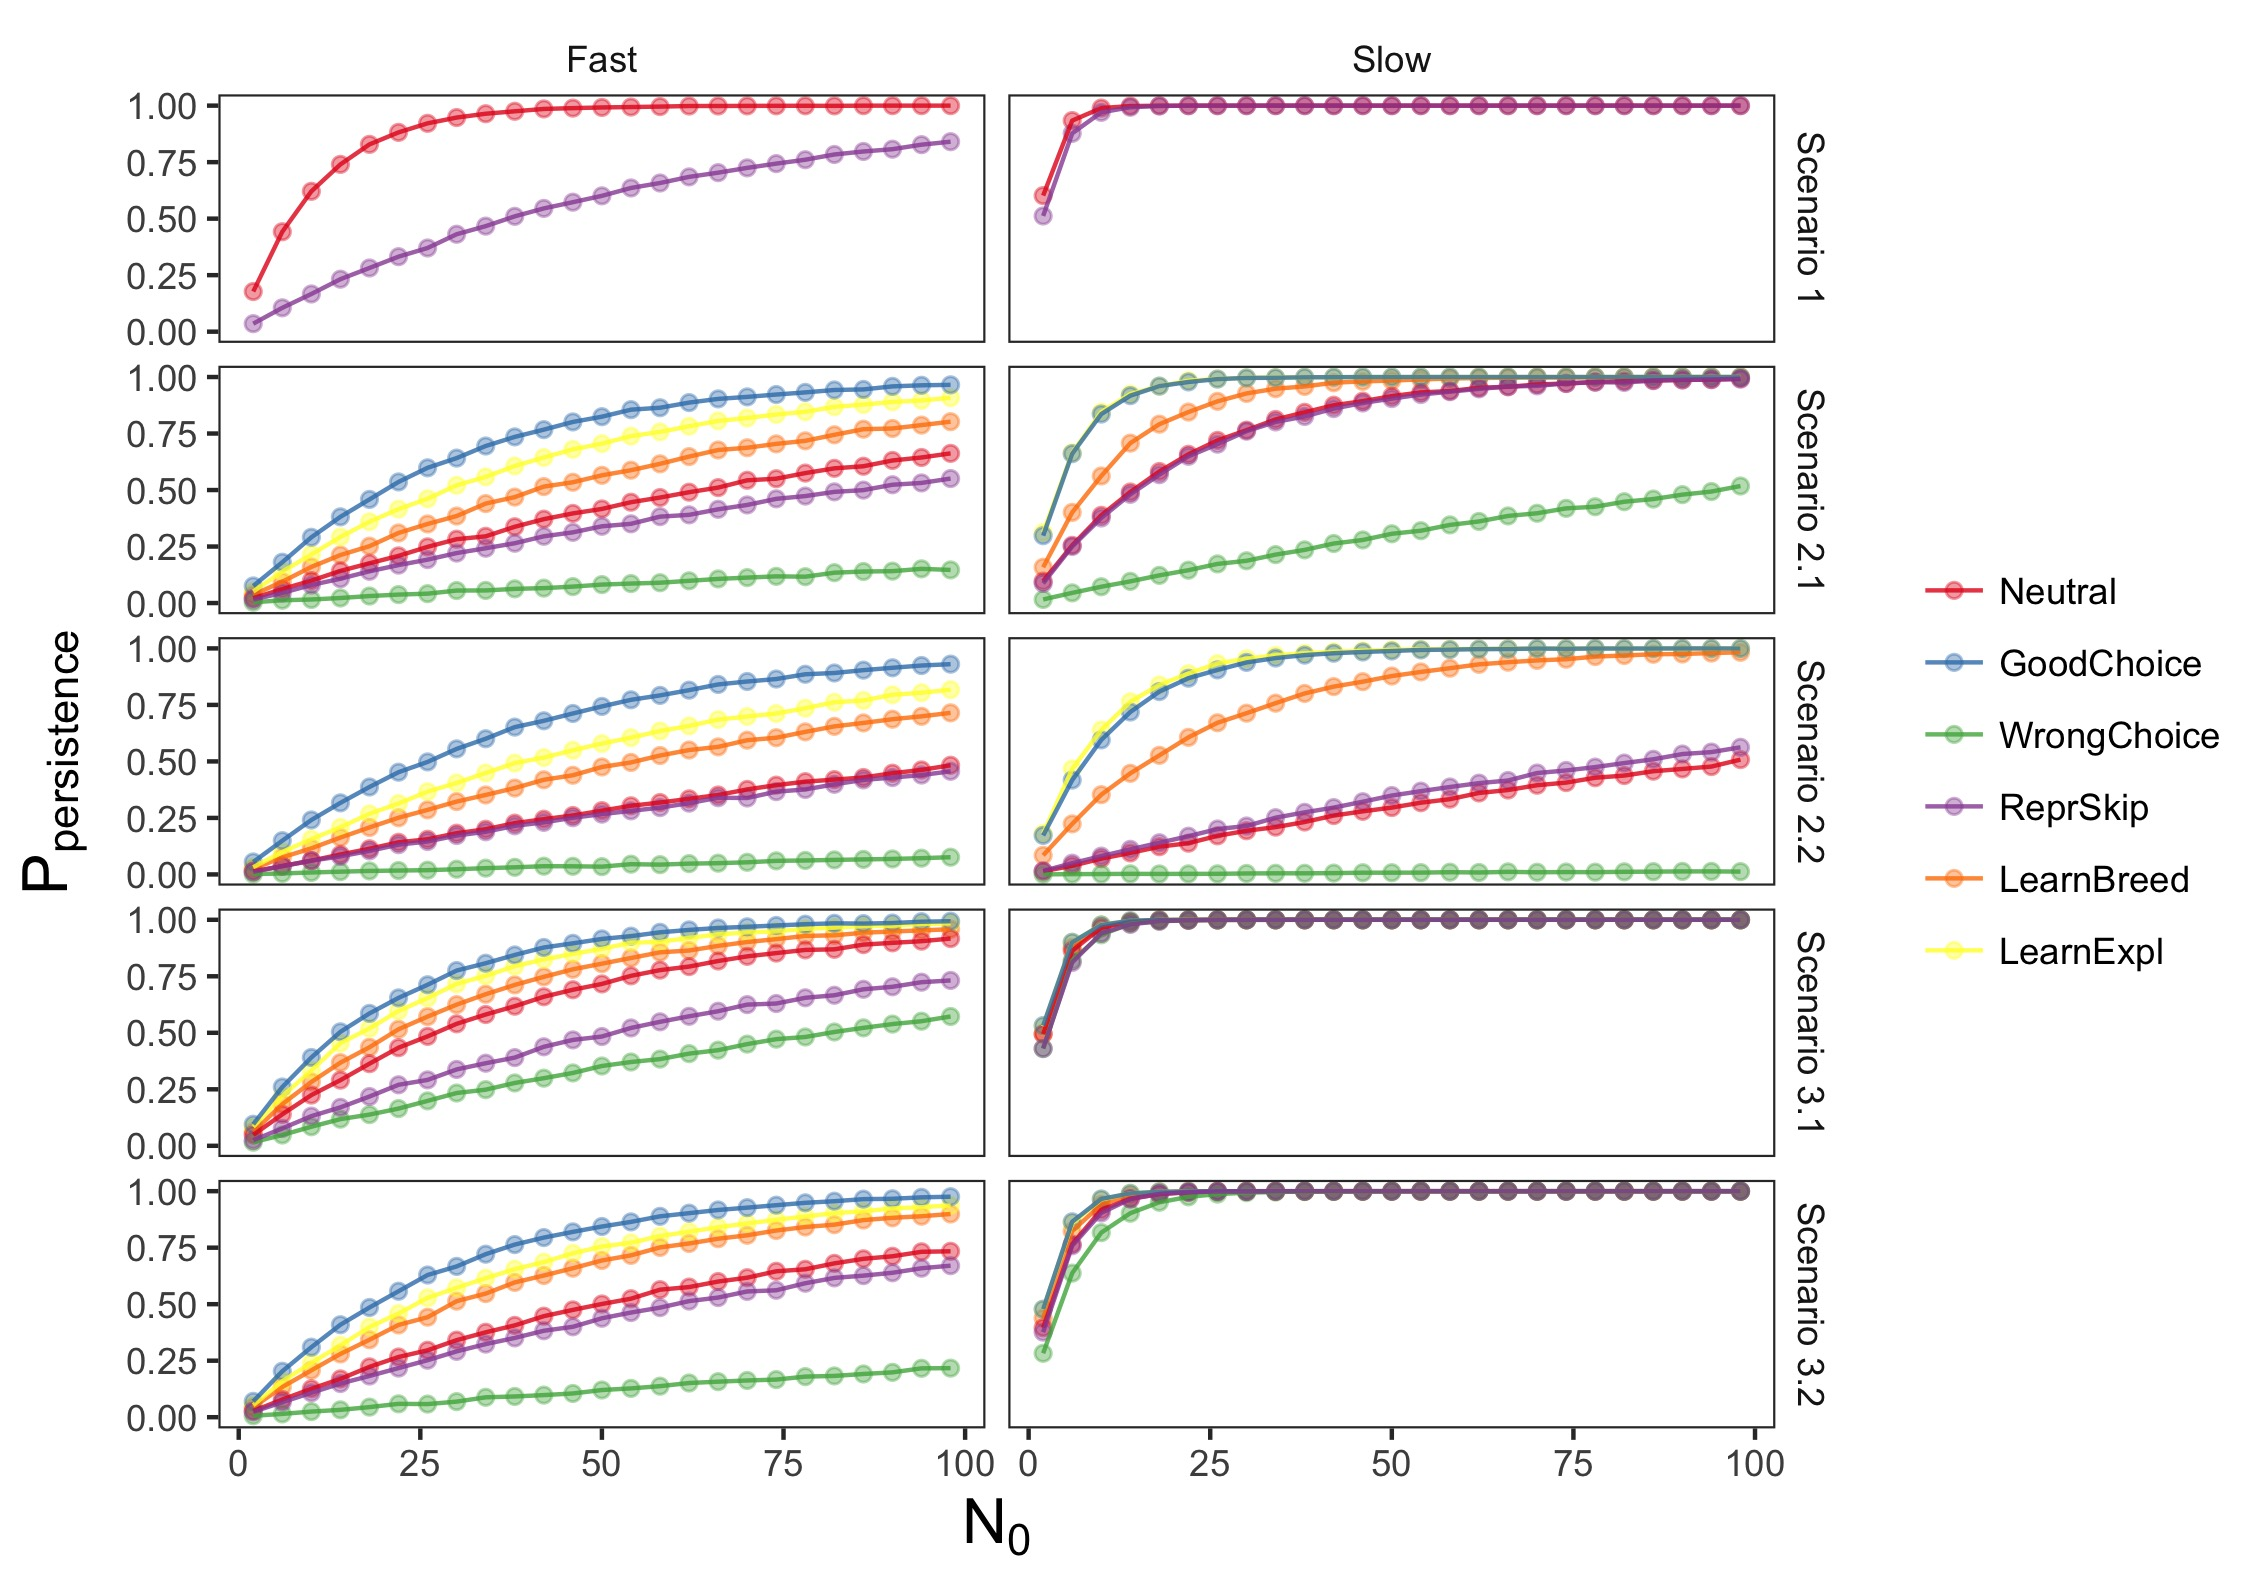
\includegraphics[width=\textwidth]{./Figures/chapter03/Fig_1.jpg}
\caption[Persistence as a function of LH, behviour and scenario]{
Simulations of probability of population persistence for 10 000 replicates as a
function of behavioural responses (\emph{Neutral}, random behavioural responses;
\emph{GoodChoice}, matching habitat choice; \emph{BadChoice}, habitat
mismatching choice; \emph{ReprSkip}, reproductive skipping; \emph{LearnExpl},
learning through exploration; \emph{LearnBreed}, learning from breeding
experience) for different initial population sizes according to different life
histories (fast and slow). Simulations have been run with the same deterministic
growth rate ($\lambda$) of 1.05 and moderate behavioural responses, under the
five different scenarios: phenotype – environmental matching (scenario 1) and
phenotype – environmental mismatch causing moderate increases of adult mortality
(scenario 2.1), extremely high adult mortality (scenario 2.2), moderate
increases of juvenile mortality (scenario 3.1) and extremely high juvenile
mortality (scenario 3.2). Simulations with strong behavioural responses are
shown in the electronic supplementary material, figure \ref{fig:figApp3.2.2}.
The fast strategy is characterized by early onset of first reproduction (1 year
old), high annual fecundity ($q = 8$) and low adult survival
($p_{1,s_{b}} = 0.4$), while the slow strategy exhibits delayed onset of
reproduction (3 years old), low fecundity ($q = 8$) and delayed onset of first
reproduction but high adult survival ($p_{1,s_{b}} = 0.85$). Note that in
scenario 1, the two habitats are the same, and therefore, all behavioural
responses except reproductive skip are equivalent to the neutral behaviour.}
\label{fig:fig3.1}
\end{figure}

We first illustrate the results of the model by presenting the
simulations for two species with the same maximum deterministic
growth rate ($\lambda = 1.05$) but striking differences in life
history, one being at the fast extreme of the fast–slow continuum
and the other at the slow extreme. Figure \ref{fig:fig3.1} presents
the simulated probability that these species thrive in a novel
environment as a function of initial population size ($N_{0}$),
according to different behavioural responses and scenarios of
maladaptation (see also the electronic supplementary material,
figure \ref{fig:figApp3.2.2}). In all the scenarios, the likelihood of establishment
increases with $N_{0}$ until reaching a threshold above which the
probability of population persistence is 1 (i.e. all simulated
populations become established). This pattern, which has
also been found empirically \citep{Blackburn2013, Sol2013}, reflects the pervasive
effect of demographic stochasticity at small population sizes.

In the absence of behavioural responses (red line), the curve
relating the probability of persistence and $N_{0}$ becomes flatter
under maladaptation (figure \ref{fig:fig3.1}, scenarios 2.1, 2.2, 3.1 and 3.2)
relative to scenarios where there is phenotype–environment
match. This is because the population not only suffers from
demographic stochasticity but also from the negative population
growth of the fraction of the population settled in the
low-quality habitat. The new route towards extinction largely
reduces population persistence, notably in scenarios where
the phenotype–environment mismatch is higher (electronic
supplementary material, figure \ref{fig:figApp3.2.2}, scenarios 2.2. and 3.2).

When individuals are allowed to take decisions, either
based on inherited or learned preferences, the probability of
persistence experiences substantial changes relative to the situation
where their behavioural responses are neutral (figure \ref{fig:fig3.1};
electronic supplementary material, figure \ref{fig:figApp3.2.2}). Matching
habitat choice and learning both contribute substantially to
increase the likelihood of persistence in a context of maladaptation.
Learning is generally not so efficient as an innate choice
based on perfect knowledge. When knowledge is imperfect,
however, innate responses can increase extinction risk by leading
individuals to choose an inappropriate habitat. Likewise,
the decision of skipping a reproductive event when conditions
are unfavourable often entails important fitness costs, reducing
the probability of establishment.


\subsection*{b) Integrating behavioural responses and life-history strategies}

\begin{figure}
\centering
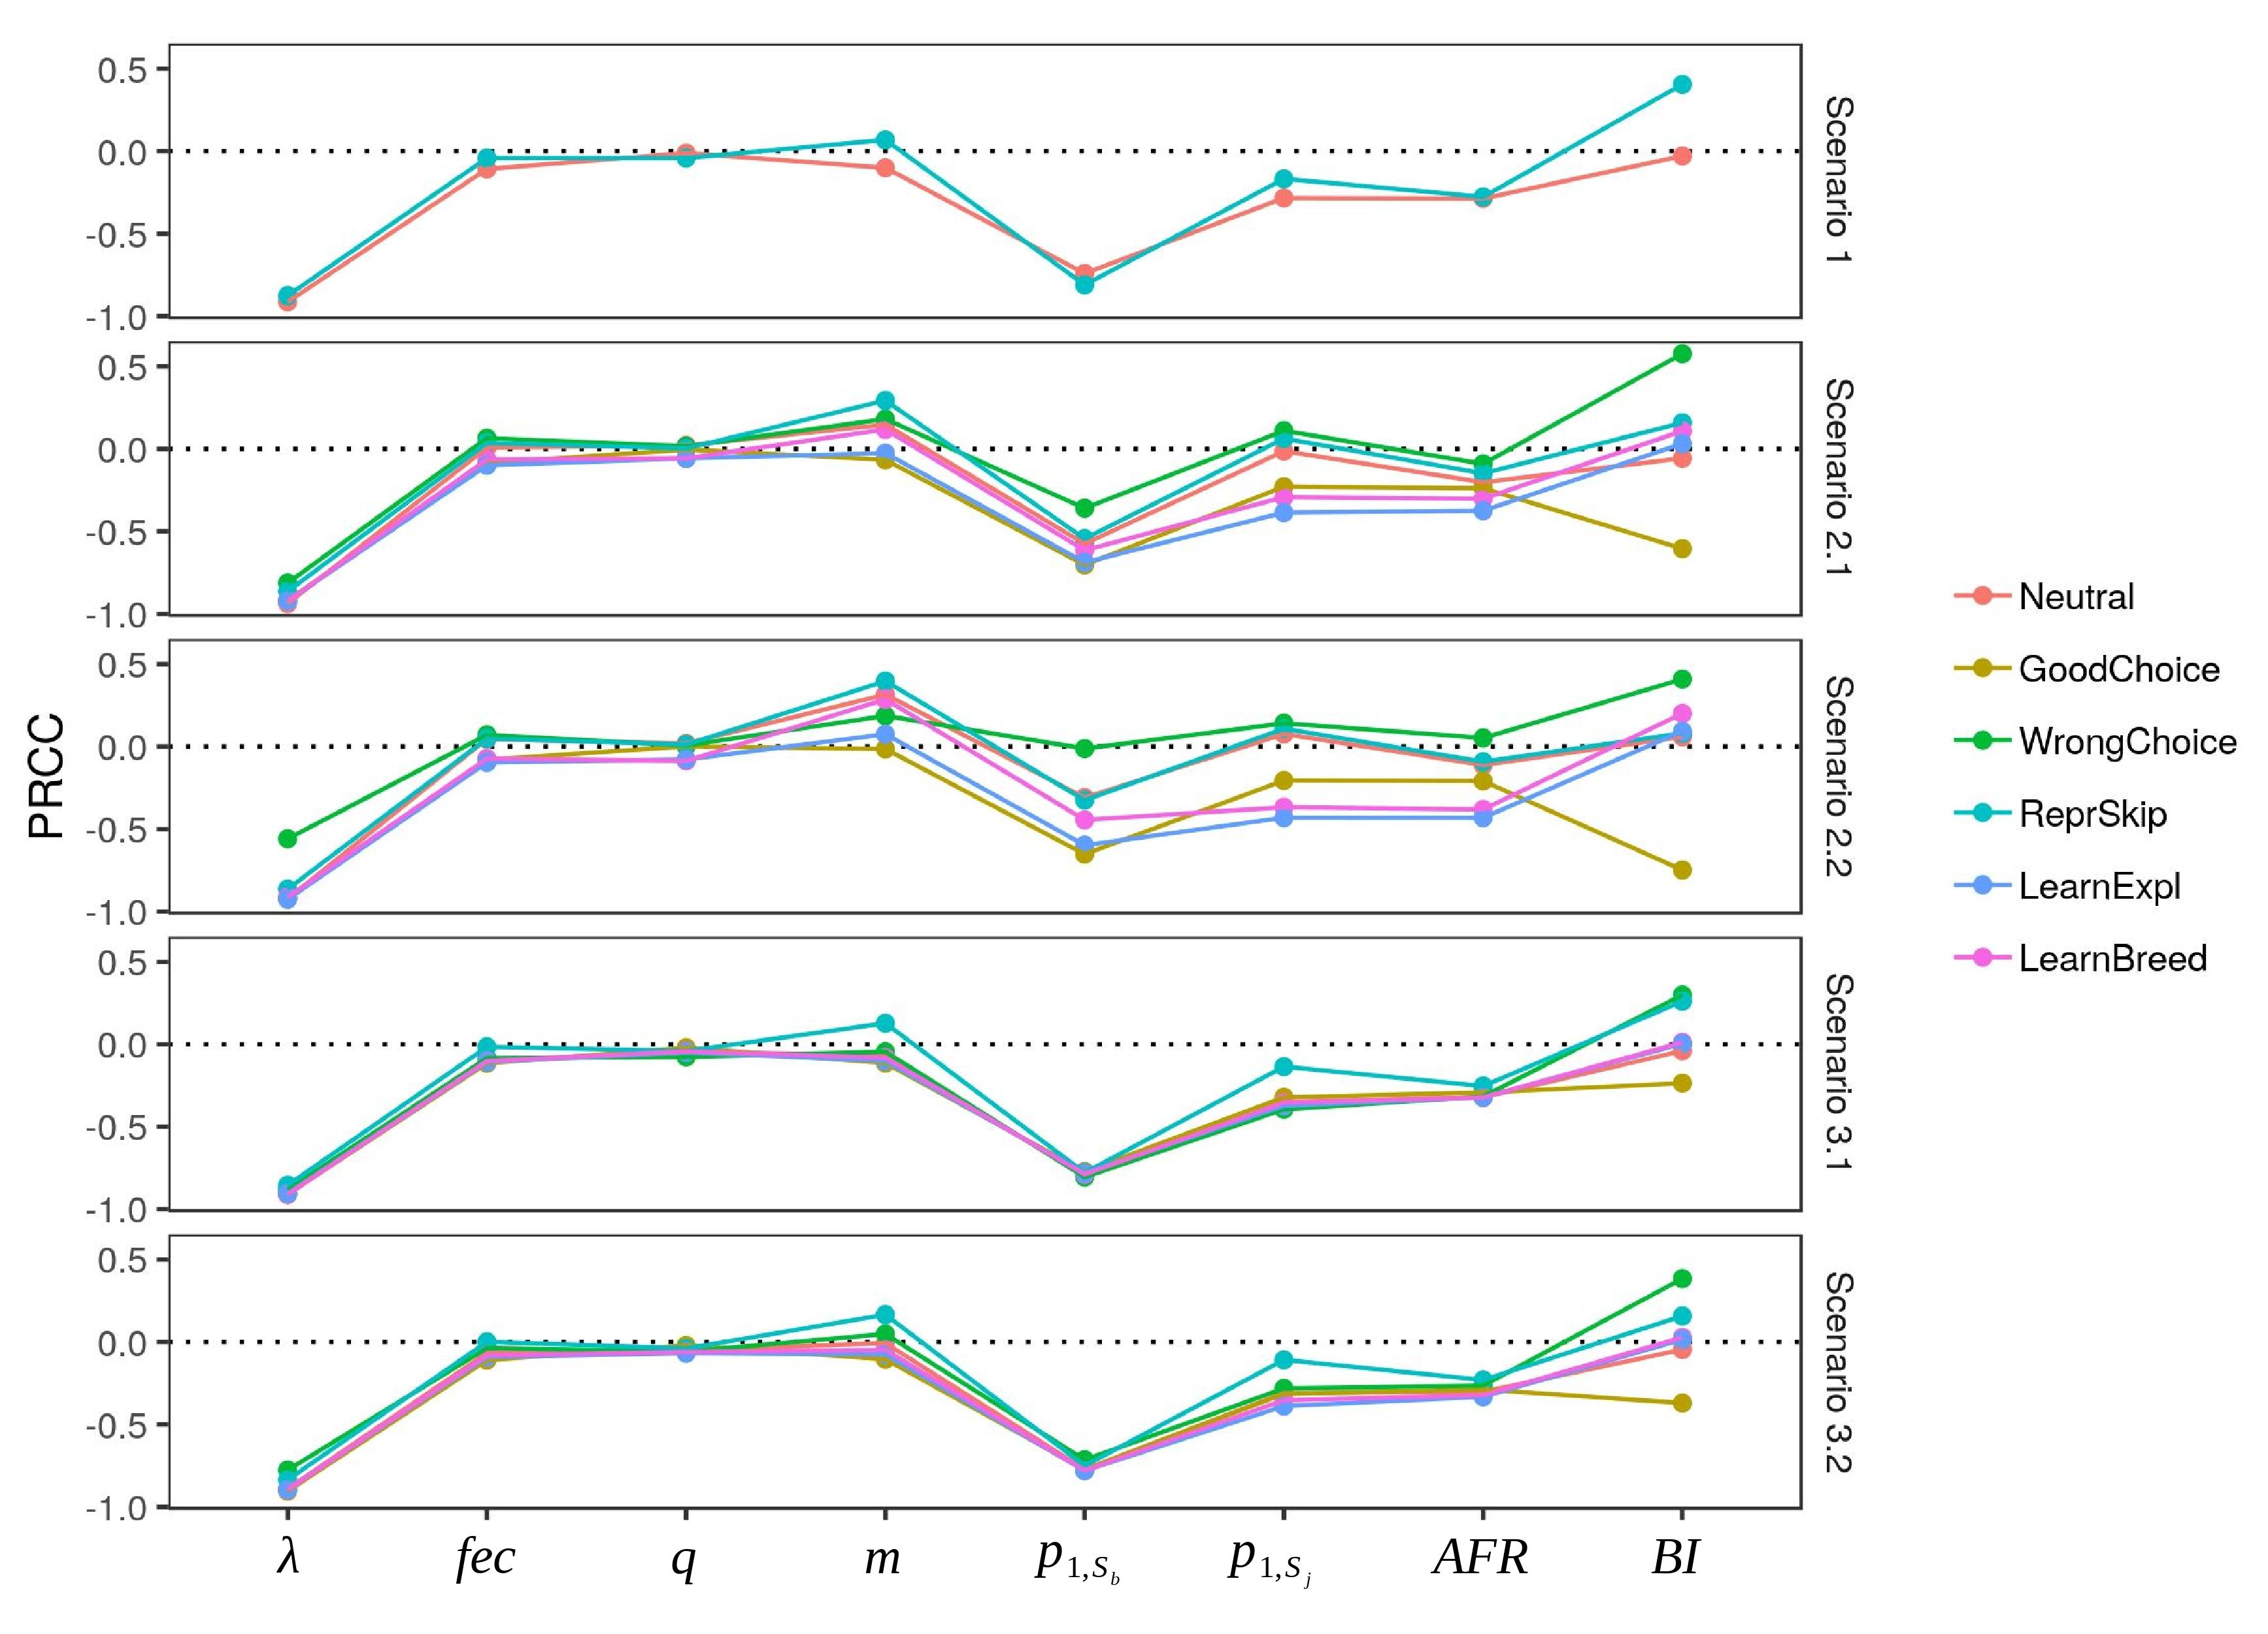
\includegraphics[width=\textwidth]{./Figures/chapter03/Fig_2.jpg}
\caption[Sensitivity of $N_{0}P_{50\%}$]{
Sensitivity of the probability of population persistence to life-history traits
for different behavioural responses and maladaptive scenarios, based on PRCC.
Population persistence is measured as $N_{0}P_{50\%}$, the initial population
that give a 50\% chance of persistence. Notation not shown in table
\ref{tab:table3.1} is as follows: $\lambda$ is the
deterministic grow rate; $fec$ is fecundity expressed as the number of offspring
produced annually ($m \cdot q$); $AFR$, is the age at first reproduction; $BI$
is the intensity of the behavioural responses, i.e. either moderate or strong.
Analyses are based on 3612 combinations of life-history traits distributing
species along the fast–slow continuum.}
\label{fig:fig3.2}
\end{figure}

Figure \ref{fig:fig3.1} suggests that the way behavioural responses influence
persistence in the novel environment differ according to the position
of the species in the fast–slow continuum. To formally
explore this, we repeated the simulations for the 3612 life-history
strategies resulting from all combinations of life-history
traits with $\lambda$ between 1.05 and 1.2 (see the section Exploration
of the parameters for details). For each life-history strategy,
we then estimated $N_{0}P_{50\%}$ to describe the likelihood that
the species persists in the novel scenario as a function of their behaviour.
Sensitive analyses across all scenarios and behavioural
strategies show that $\lambda$ is the most important factor facilitating
population persistence in the novel environments (figure \ref{fig:fig3.2}).
Life-history strategies with higher $\lambda$ show lower $N_{0}P_{50\%}$, implying
that they need fewer individuals to become established.
However, adult survival is the life-history trait with greater
influence in population persistence, suggesting that slow strategies
have generally higher chances than fast strategies to
persist in novel environments (figure \ref{fig:fig3.2}). The high persistence
of slow species in novel environments does not merely result
from the individuals initially introduced being able to survive
the entire simulation period. The explored life-history trait combinations
rarely allow individuals to survive 50 years, and in
most cases, the final population is higher than the initial one
(electronic supplementary material, figure \ref{fig:figApp3.2.3}).


\subsection*{c) Costs and benefits of behavioural responses in fast and slow strategies}

\begin{figure}
\centering
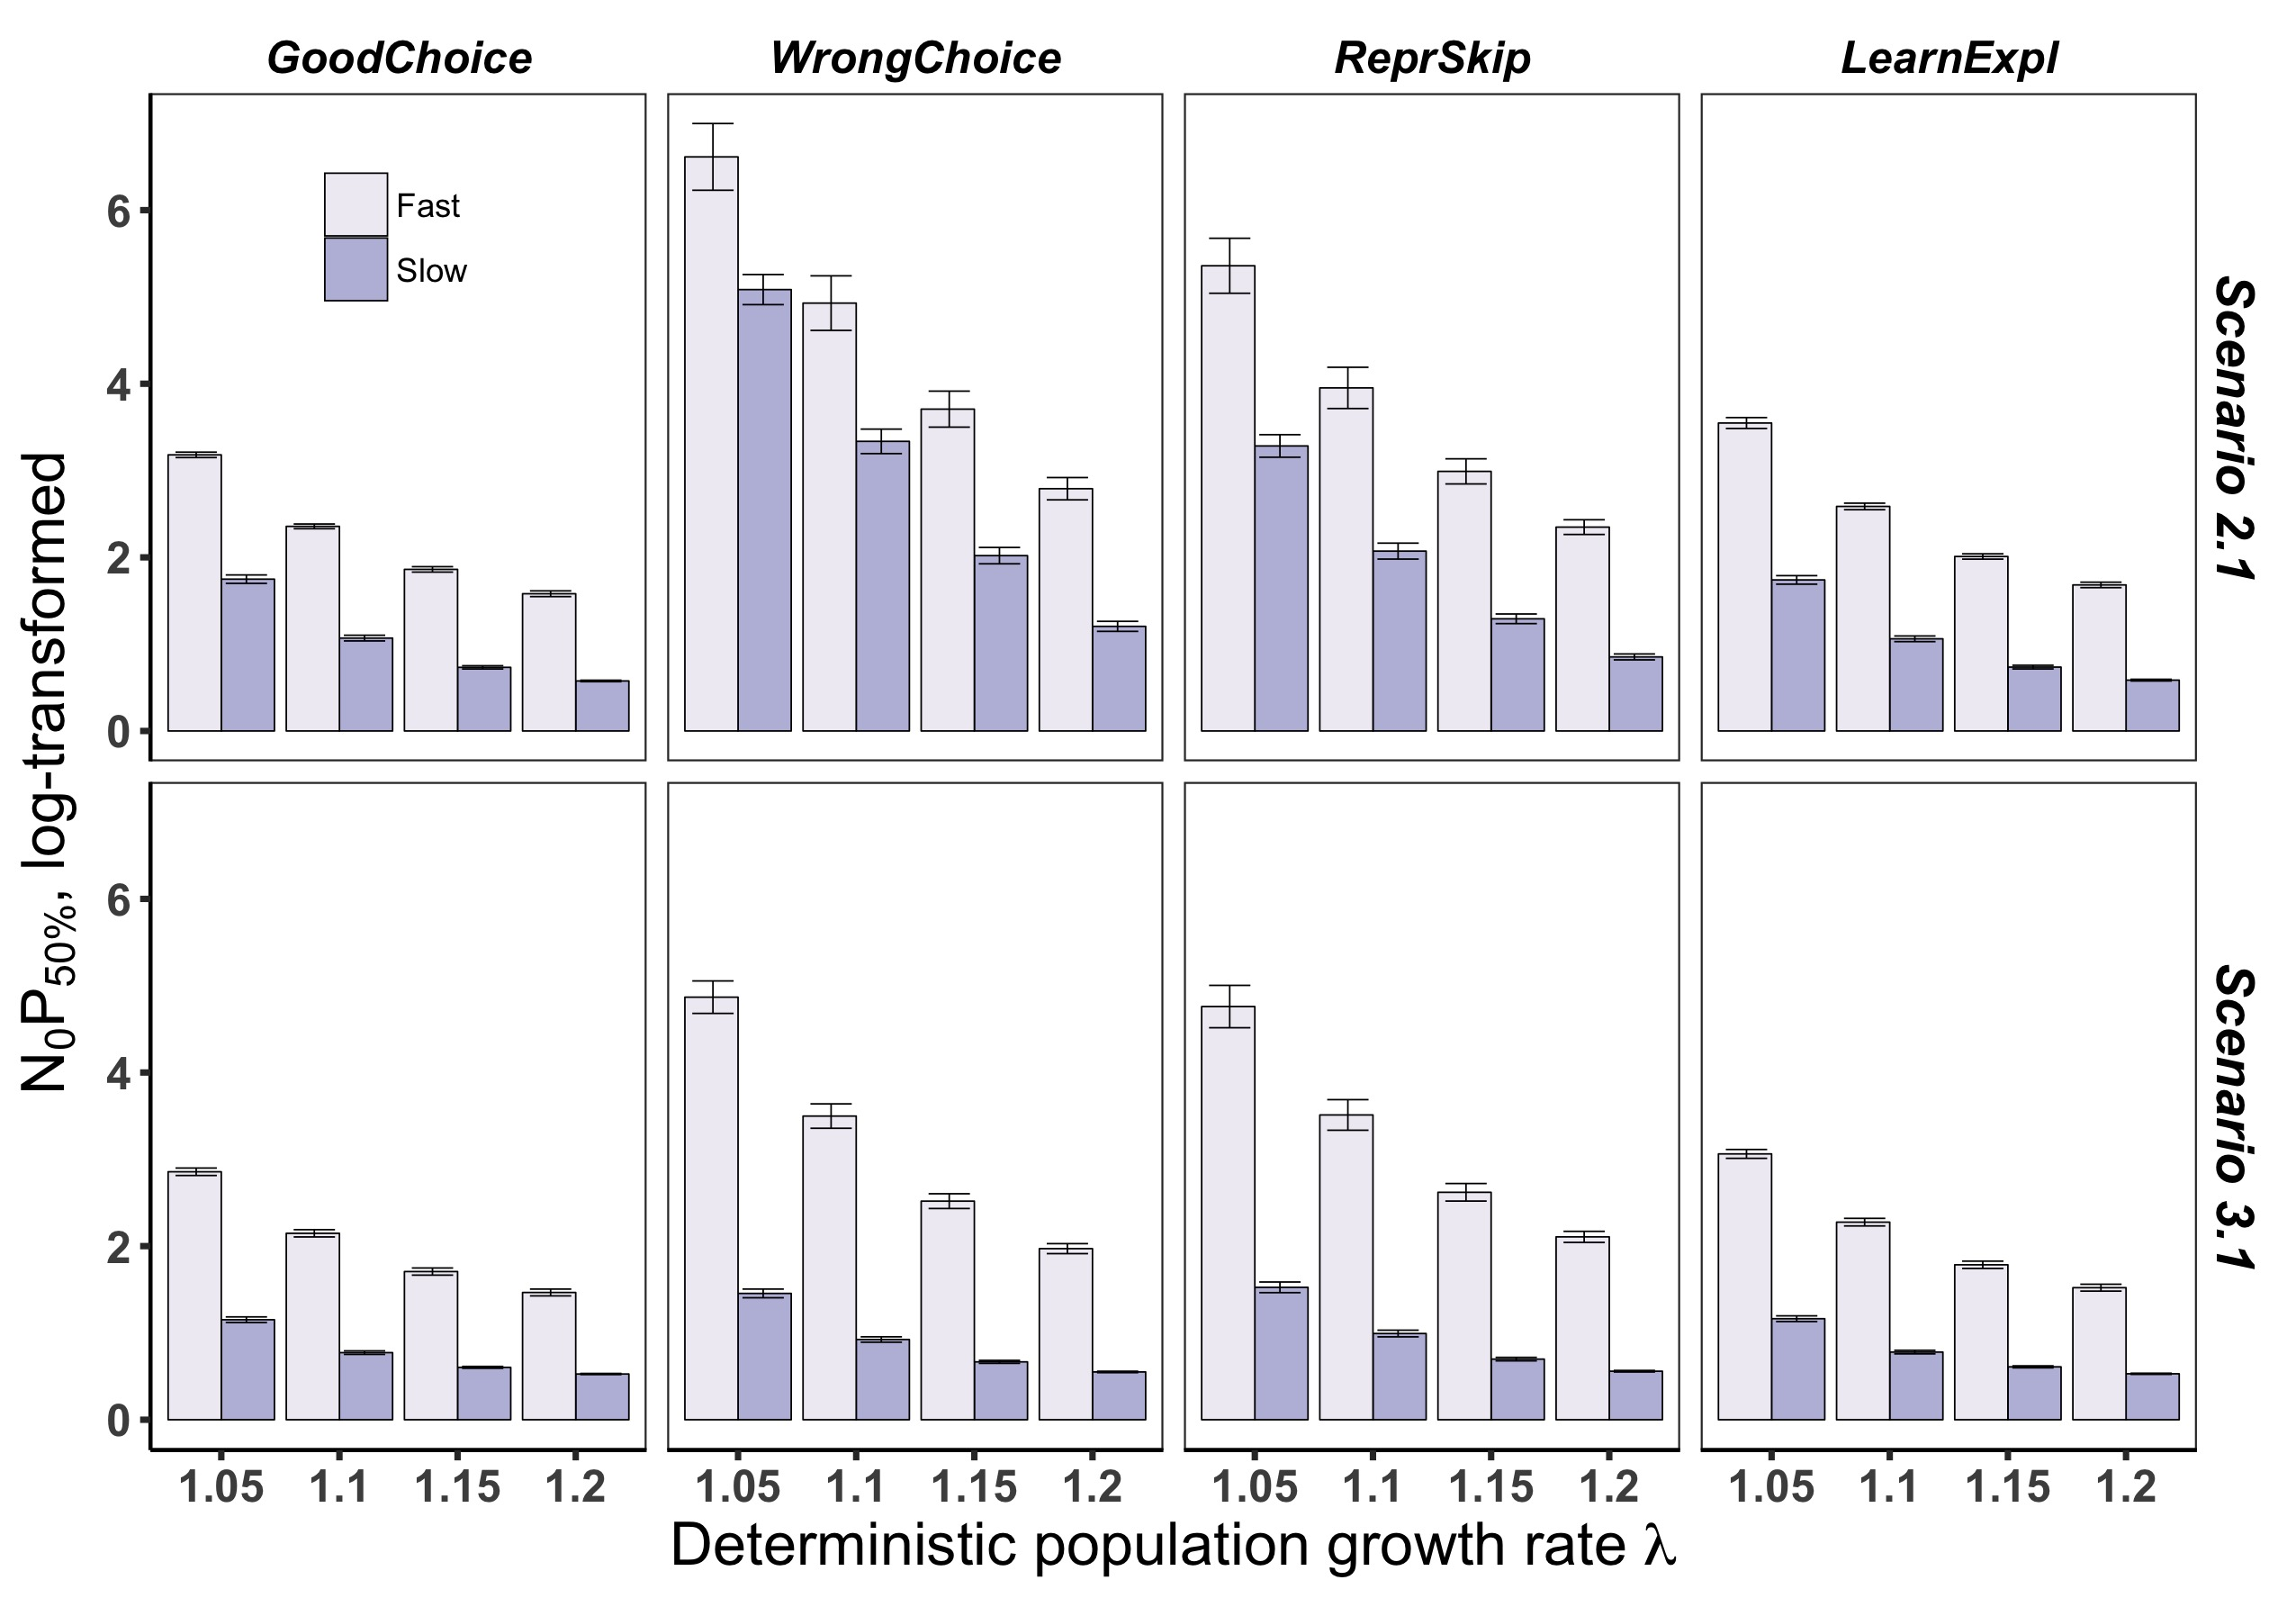
\includegraphics[width=\textwidth]{./Figures/chapter03/Fig_3.jpg}
\caption[Effects on $N_{0}P_{50\%}$]{
Effects of behavioural responses on population persistence in novel environments
as a function of the position of the animal along the fast–slow continuum.
Population persistence is estimated as $N_{0}P_{50\%}$ and behavioural responses
are moderate (for strong responses, see the electronic supplementary material,
figure \ref{fig:figApp3.2.4}). For details on abbreviations, see figure
\ref{fig:fig3.1}.}
\label{fig:fig3.3}
\end{figure}

To further investigate the interaction between behaviour and
life history, we compared life-history strategies positioned
either at the fast or slow extremes of the fast – slow continuum
(see the section Exploration of the parameters for details). The
results confirm that slow strategies generally need a lower
$N_{0}P_{50\%}$ than fast strategies to persist in the novel environments
(figure \ref{fig:fig3.3}). To reach a success similar to that of slow strategies,
fast strategies must have values of $\lambda$ substantially higher (often
more than 15\% higher) than those of slow strategies.

Under maladaptive scenarios, the probability of persistence
depends on whether the phenotype–environment mismatch
mainly affects offspring or adults, as fast and slow strategies
differ in their sensitivity to changes in fecundity and adult mortality.
Thus, although the general tendency of slow species to
be superior invaders is consistent across environmental scenarios,
slow species are particularly affected by scenarios
increasing adult mortality and fast species by those affecting
offspring mortality.

The benefits and costs of the behavioural responses are
also contingent to the position of the species along the fast –
slow continuum (figure \ref{fig:fig3.3}; electronic supplementary material,
figures \ref{fig:figApp3.2.6}–\ref{fig:figApp3.2.10}). In slow species, the gains of learning are substantial
when maladaptation increases adult mortality, while
the gains are almost negligible when maladaptation affects offspring
because they are already well protected for their life
history. Because slow strategies have more opportunities to
reproduce in the future, they are less penalized than fast
species by mistakenly choosing an inappropriate habitat to
reproduce. Likewise, the decision of skipping a reproductive
event when conditions are unfavourable, which is generally
costly (figure \ref{fig:fig3.1}), has a negligible impact on the demography
of slow species when the risk of reproductive failure is high.

For fast species, learning through exploration and an innate
preference for the high-quality habitat tend to improve population
persistence in all scenarios, although the gains are
modest and rapidly decrease at higher $\lambda$ values (figure \ref{fig:fig3.3}; electronic
supplementary material, figures \ref{fig:figApp3.2.6} and \ref{fig:figApp3.2.8}). Learning
from a reproductive failure is marginally beneficial only when
phenotype–environment match increases offspring survival,
even though the risk of extinction remains high (electronic
supplementary material, figure \ref{fig:figApp3.2.9}). The costs of preferring a
low-quality habitat or skipping a reproductive event are also
generally high in most scenarios, compared to those of slow
species, and generally cannot be compensated by increasing
$\lambda$ (electronic supplementary material, figure \ref{fig:figApp3.2.7}).


\section{Discussion}

Our results show strong support for the notion that behavioural
responses interact with life history to influence persistence in
novel environments. Under maladaptive scenarios, where the
match of the phenotype to the environment is insufficient,
the simulations suggest that it pays to have a slow life history
that increase the value of adults over the value of offspring
even at the cost of decreasing reproduction. This is in part
owing to the demographic consequences of the life-history
strategy itself and in part owing to the added benefits of behavioural
responses. Thus, a slow strategy represents a strong
buffer against maladaptation causing high offspring mortality,
indirectly affecting adult survival and hence the opportunities
for future reproduction. Instead, behavioural responses primarily
buffer individuals against maladaptation causing high
adult mortality. As novel environments are likely to increase
both adult and offspring survival, the complementary effects
of behavioural responses and life history make slow animals
particularly well equipped to cope with sudden changes in
the environment.

The notion that slow animals exposed to novel environments
generally gain greater benefits from behavioural responses has
been suggested in previous studies. Animals at the ‘slow’
extreme of the fast–slow continuum are generally believed to
explore more accurately the environment and exhibit better performance
in learning than those at the ‘fast’ extreme (reviewed in \citet{Sol2016}).
\citet{Eliassen2007}, for instance, developed a model to investigate
how foragers benefit from using a simple learning rule to
update estimates of temporal changes in resource levels; the
model showed that as lifetime expectancy decreases, learners
invest less in information acquisition and show lower foraging
performance when resource level changes through time. Our
simulations generally align with these studies, even though we
did not explicitly consider cognitive differences in learning
between fast and slow animals. Although it is likely that including
these differences accentuate the superiority of slow species in
contexts of maladaptation, this will depend on costs that are difficult
to estimate. Our model assumes some costs of behavioural
responses, such as imperfect information leading to choose a
low-quality habitat and a loss of breeding opportunities. However,
there are other costs not considered, such as those related
to the need to invest time and energy to produce and maintain
the neural and cognitive functions needed to acquire and
respond to environmental information.

A particularly intriguing question is to what extent innate
preferences and learning interact to influence the realized
preferences for habitats. \citet{Kawecki2010} argued that an individual
with no clear innate preference will be more amenable to
changing its preference as a result of experience than an individual
that already shows a strong innate preference, even
when it means choosing a low-quality resource. Thus, it
may be that some species primarily rely on matching the
environment to the phenotype through habitat matching
choice, while others rely more on improving the match of the
phenotype to the new environment through learning. Several
factors might contribute to favour one strategy over the other.
Natural selection on heritable variation in habitat preferences
should be more efficient in fast species, whose short generation
times increase mutation rates and changes in allele
frequency. Instead, in slow species that respond more
slowly to selection, learned preferences would outperform
genetically determined preferences (present study, see also \citet{Kokko2001}).
Learning might also be particularly favoured in ecological
generalists. A generalist strategy selects against local
adaptation \citep{Kisdi2002}, and frequently exposes individuals to new
challenges that require learned responses \citep{Sol2016a, Ducatez2015}. Our
simulations suggest an additional factor that might contribute to
favour learning over phenotype matching choice: the degree
of novelty in the environment. We find that learning does
not avoid extinctions as efficiently as perfect knowledge,
but in terms of population persistence, it avoids the risk of
falling into an ecological trap. Learning seems thus to be a
better strategy than matching habitat choice to thrive in
environments that are very different from the ancestral
environments or that change too fast to provide reliable
cues for habitat choice. One example could be urban environments.
These environments expose animals to a variety of
challenges that are drastically different from those found in
nature, such as the need to confront frequent disturbances
by people or avoid risks associated with traffic and buildings.
Growing evidence indicate that urban animals tend to be
more proficient in learning than non-urban animals \citep{Sol2013a}.

Our results contribute to the debate over whether successful
invaders should be characterized as fast or slow, an issue of
high relevance to predict and prevent the spread and impact of
biological invasions. Although life history has long been
deemed essential to understanding the success of invaders
\citep{Lewontin1969}, confidence in theoretical arguments has been undermined
by a perceived lack of empirical support \citep{Sol2012a}. The dissociation
between theoretical and empirical work has in part been attributed
to the excessive focus on the ‘small population paradigm’
\citep{Sol2016}, which assumes that demographic stochasticity is the main
driver of extinction in introduced populations. This has led to
the widespread belief that successful invaders are characterized
by high fecundity that reduces the risk of stochastic
extinctions by facilitating rapid population growth from
small initial populations. While this process has received
some empirical support \citep{Allen2017, Capellini2015}, our results align with theoretical
and empirical work suggesting that it mainly applies when
the organism’s phenotype matches well with the environment
\citep{Sol2012a, Jeppsson2012}. Yet, under maladaptive scenarios our simulations
indicate that fast strategies are more affected by ecological traps
and are only superior to slow strategies when their population
growth rate is substantially higher. Moreover, this superiority
is only noticeable when the phenotype mismatch with the
environment increases adult mortality, reflecting that population
growth of fast species is less sensitive to changes in
adult mortality than in fecundity. Given the importance of parental
care in many animals, however, it is unrealistic to assume
that a high adult mortality will not be accompanied by
increased offspring mortality \citep{Santema2018}. The crucial question is
therefore to what extent fast animals can maintain high population
growth rates in a context of maladaptation. Current evidence
in birds and mammals does not indicate that fast species
have higher population growth rates in the wild than slow-lived
species (electronic supplementary material, figure \ref{fig:figApp3.2.11}).
To properly clarify this issue on empirical grounds, however,
we would need field estimations of population growth rate
for fast and slow populations exposed to different degrees of
phenotype–environment mismatch. Unfortunately, this type
of information is currently unavailable.

As any model, ours is a simplified representation of the reality.
An issue that remains insufficiently resolved is how different
behavioural responses affect establishment success when acting
in concert. In our simulations, we have investigated behavioural
mechanisms separately, to be able to disentangle their effects, but
in reality, it is likely that they act in concert, either synergically or
antagonistically. The challenge here is to parametrize the models
in a way that is realistic enough to avoid biasing the simulations,
but this requires a better understanding of mechanisms. Another
issue that will need further attention in the future is the possibility
that other mechanisms in addition of those analysed here
also influence the response to environmental changes. We have
previously suggested that producing several broods in the
same breeding season can afford high benefits when the chances
of a reproductive failure are high, as it provides the advantage of
a high annual fecundity while reducing the costs of a reproductive
failure \citep{Sol2012a}. Future models will also have to consider Allee
effects, that is, the decline in the rates of reproduction and/or survival
at low population densities. These effects are not only
highly relevant during the early stages of the invasion process,
but may also be tied to the life history and behavioural strategies
of the species \citep{Leung2004}. A preference for a low-quality habitat is
indeed a type of Allee effect, as it slows population growth at
low densities \citep{Kokko2001}, but other types of Allee effects could also be relevant
\citep{Reznick2002}. Allee effects are expected to be particularly relevant in
highly social animals that rely more on social and public information
to take decisions and learn. Advancing in all these
themes will offer a more complete picture of how animals cope
with environmental changes.

Although organisms that are slow-lived relative to the rate
of environmental fluctuations often exhibit enhanced learning
abilities \citep{Sol2016a}, the evolutionary causes are less well understood.
It has been suggested that the causal link between learning and
longevity could be bi-directional \citep{Eliassen2007, Ratikainen2019, Sol2009a}. The possibility of
constructing behavioural responses to ecological challenges
might directly affect the evolution of life histories by buffering
individuals from extrinsic mortality. The evolved combination
of life-history traits might in turn alter the fitness benefits and
costs of behavioural responses, as suggested here. However,
the covariation between learning and life history can also
result from correlated evolution \citep{Sol2016a}. Our results reinforce
this latter view, suggesting that the environments which
favour slow life-history strategies are similar to those favouring
learning. Thus, behavioural plasticity and slow life histories
might be dimensions of a same pace-of-life syndrome to cope
with sudden environmental changes \citep{Sol2016a}.

We have shown that considering variation in life-history
species is relevant when predicting the influence of behaviour
on the probability of persisting in novel environments.
Although the interplay between behaviour and life history
is still insufficiently understood, our results highlight that
to continue advancing, we need to acknowledge that both
may be part of a broader adaptive system of organisms to
cope with rapid environmental changes.
